\localauthor{Thomas Kirz}

\subsection{Hochladen einer Revision}\label{subsec:sequenz-revision-hochladen}

Abbildung~\ref{fig:upload-revision-sequence} zeigt die Interaktionen zwischen den Klassen beim Ablehnen einer Einreichung.

\begin{figure}
    \centering
    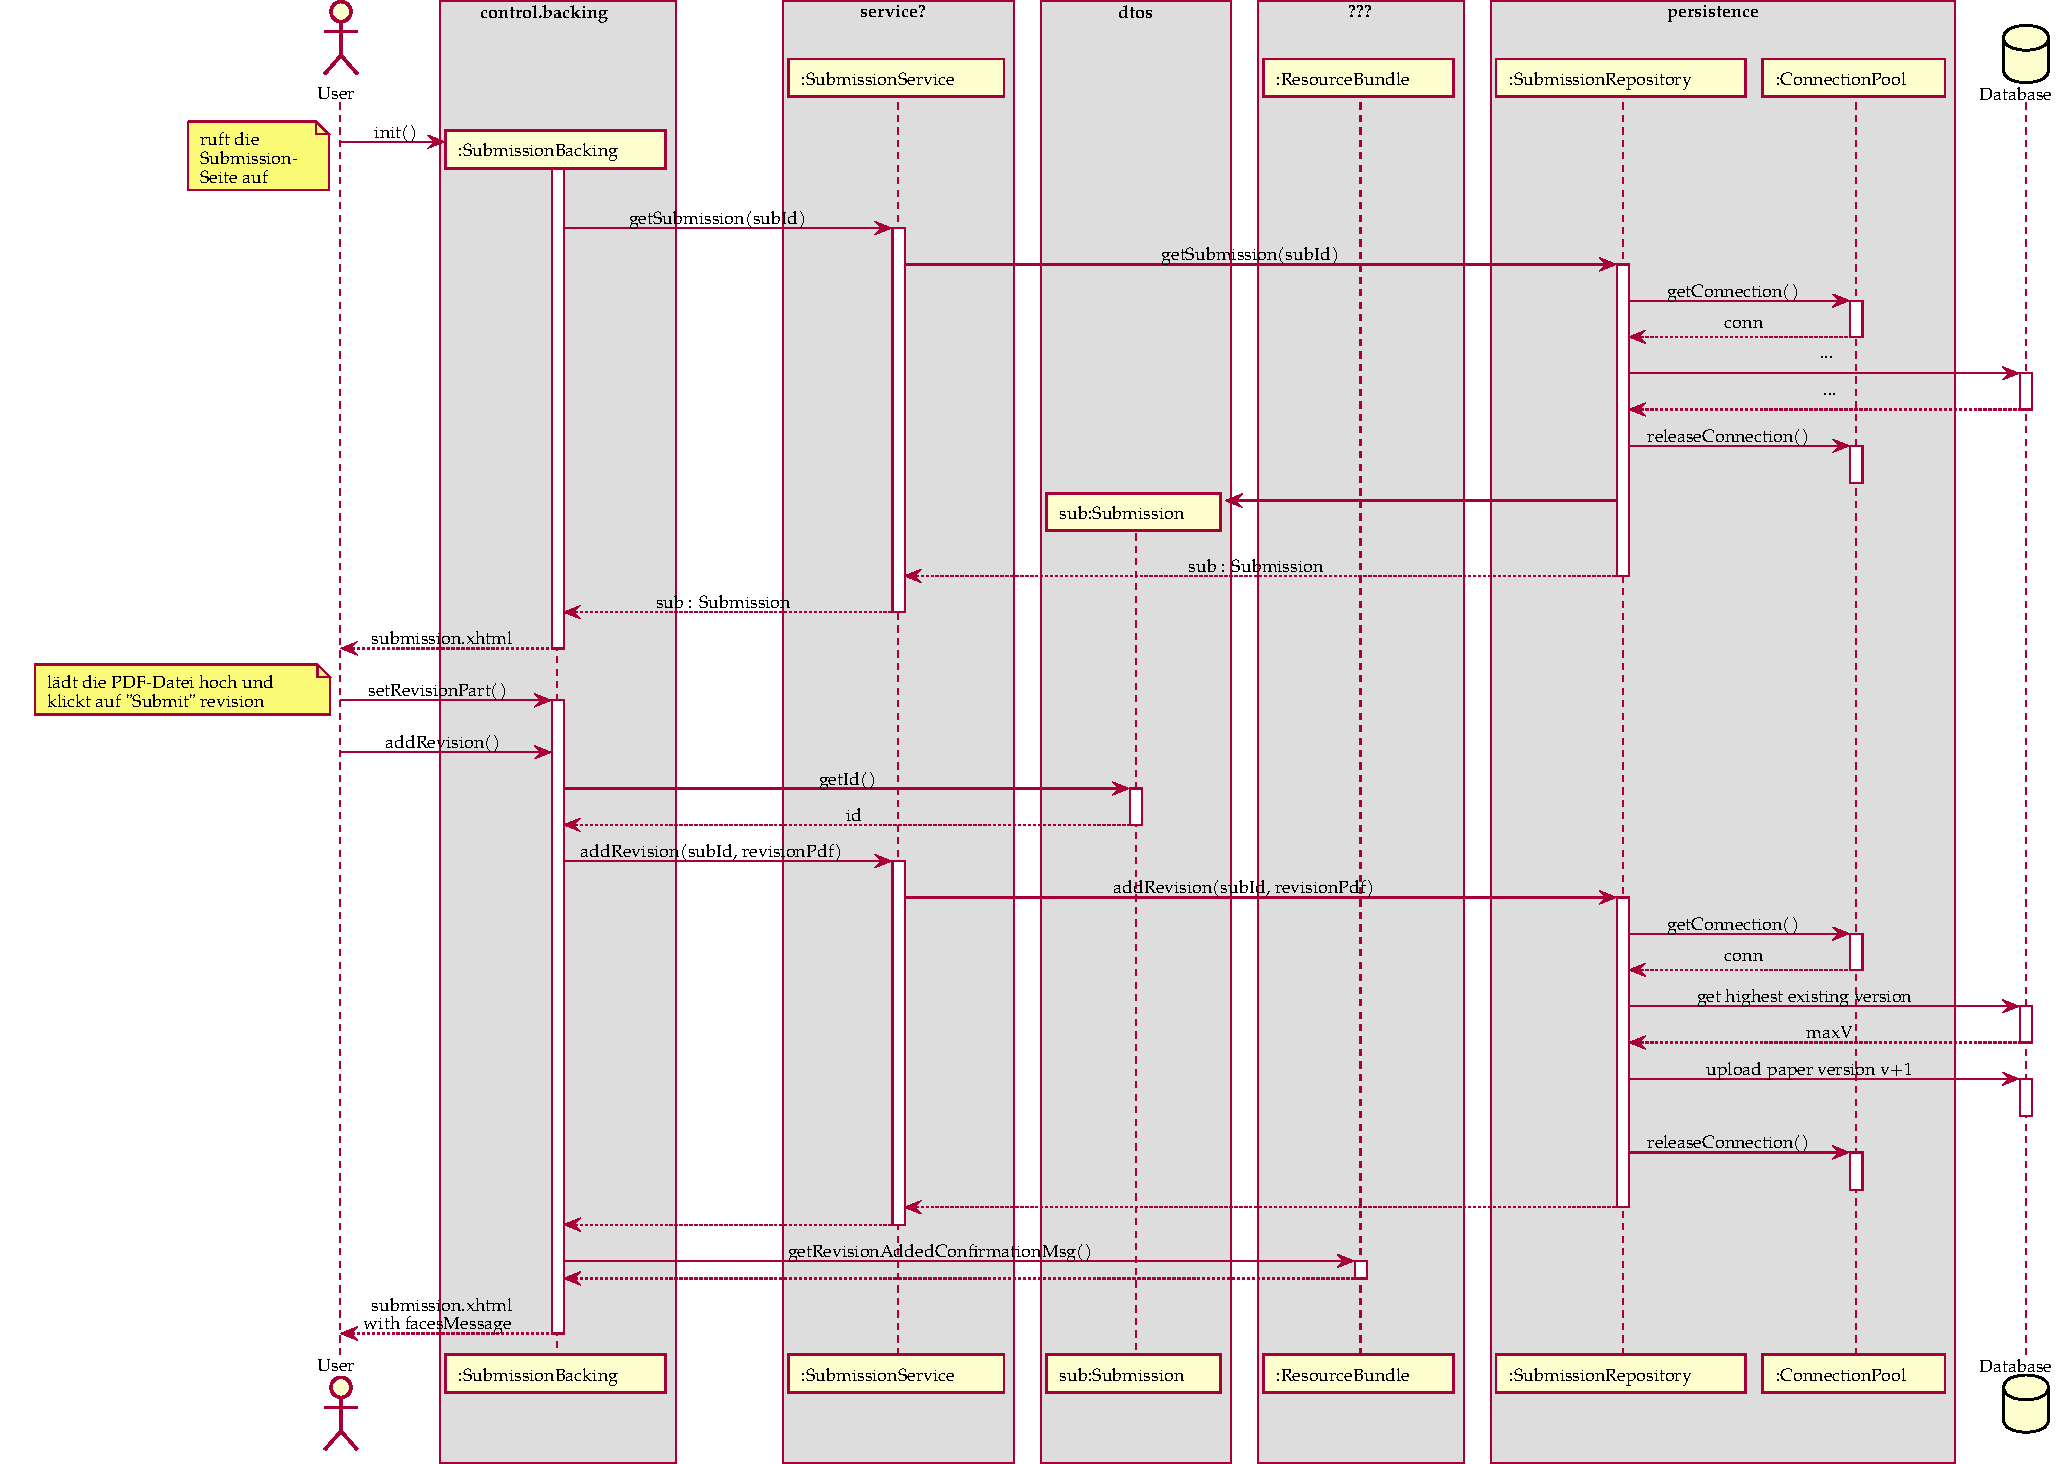
\includegraphics[width=\textwidth]{graphics/upload_revision}
    \caption{Sequenzdiagramm zur Ablehnung einer Einreichung}
    \label{fig:upload-revision-sequence}
\end{figure}

\subsection{Ablehnung einer Einreichung}\label{subsec:sequenz-ablehnung}

Abbildung~\ref{fig:rejection-sequence} zeigt die Interaktionen zwischen den Klassen beim Ablehnen einer Einreichung.

\begin{figure}
    \centering
    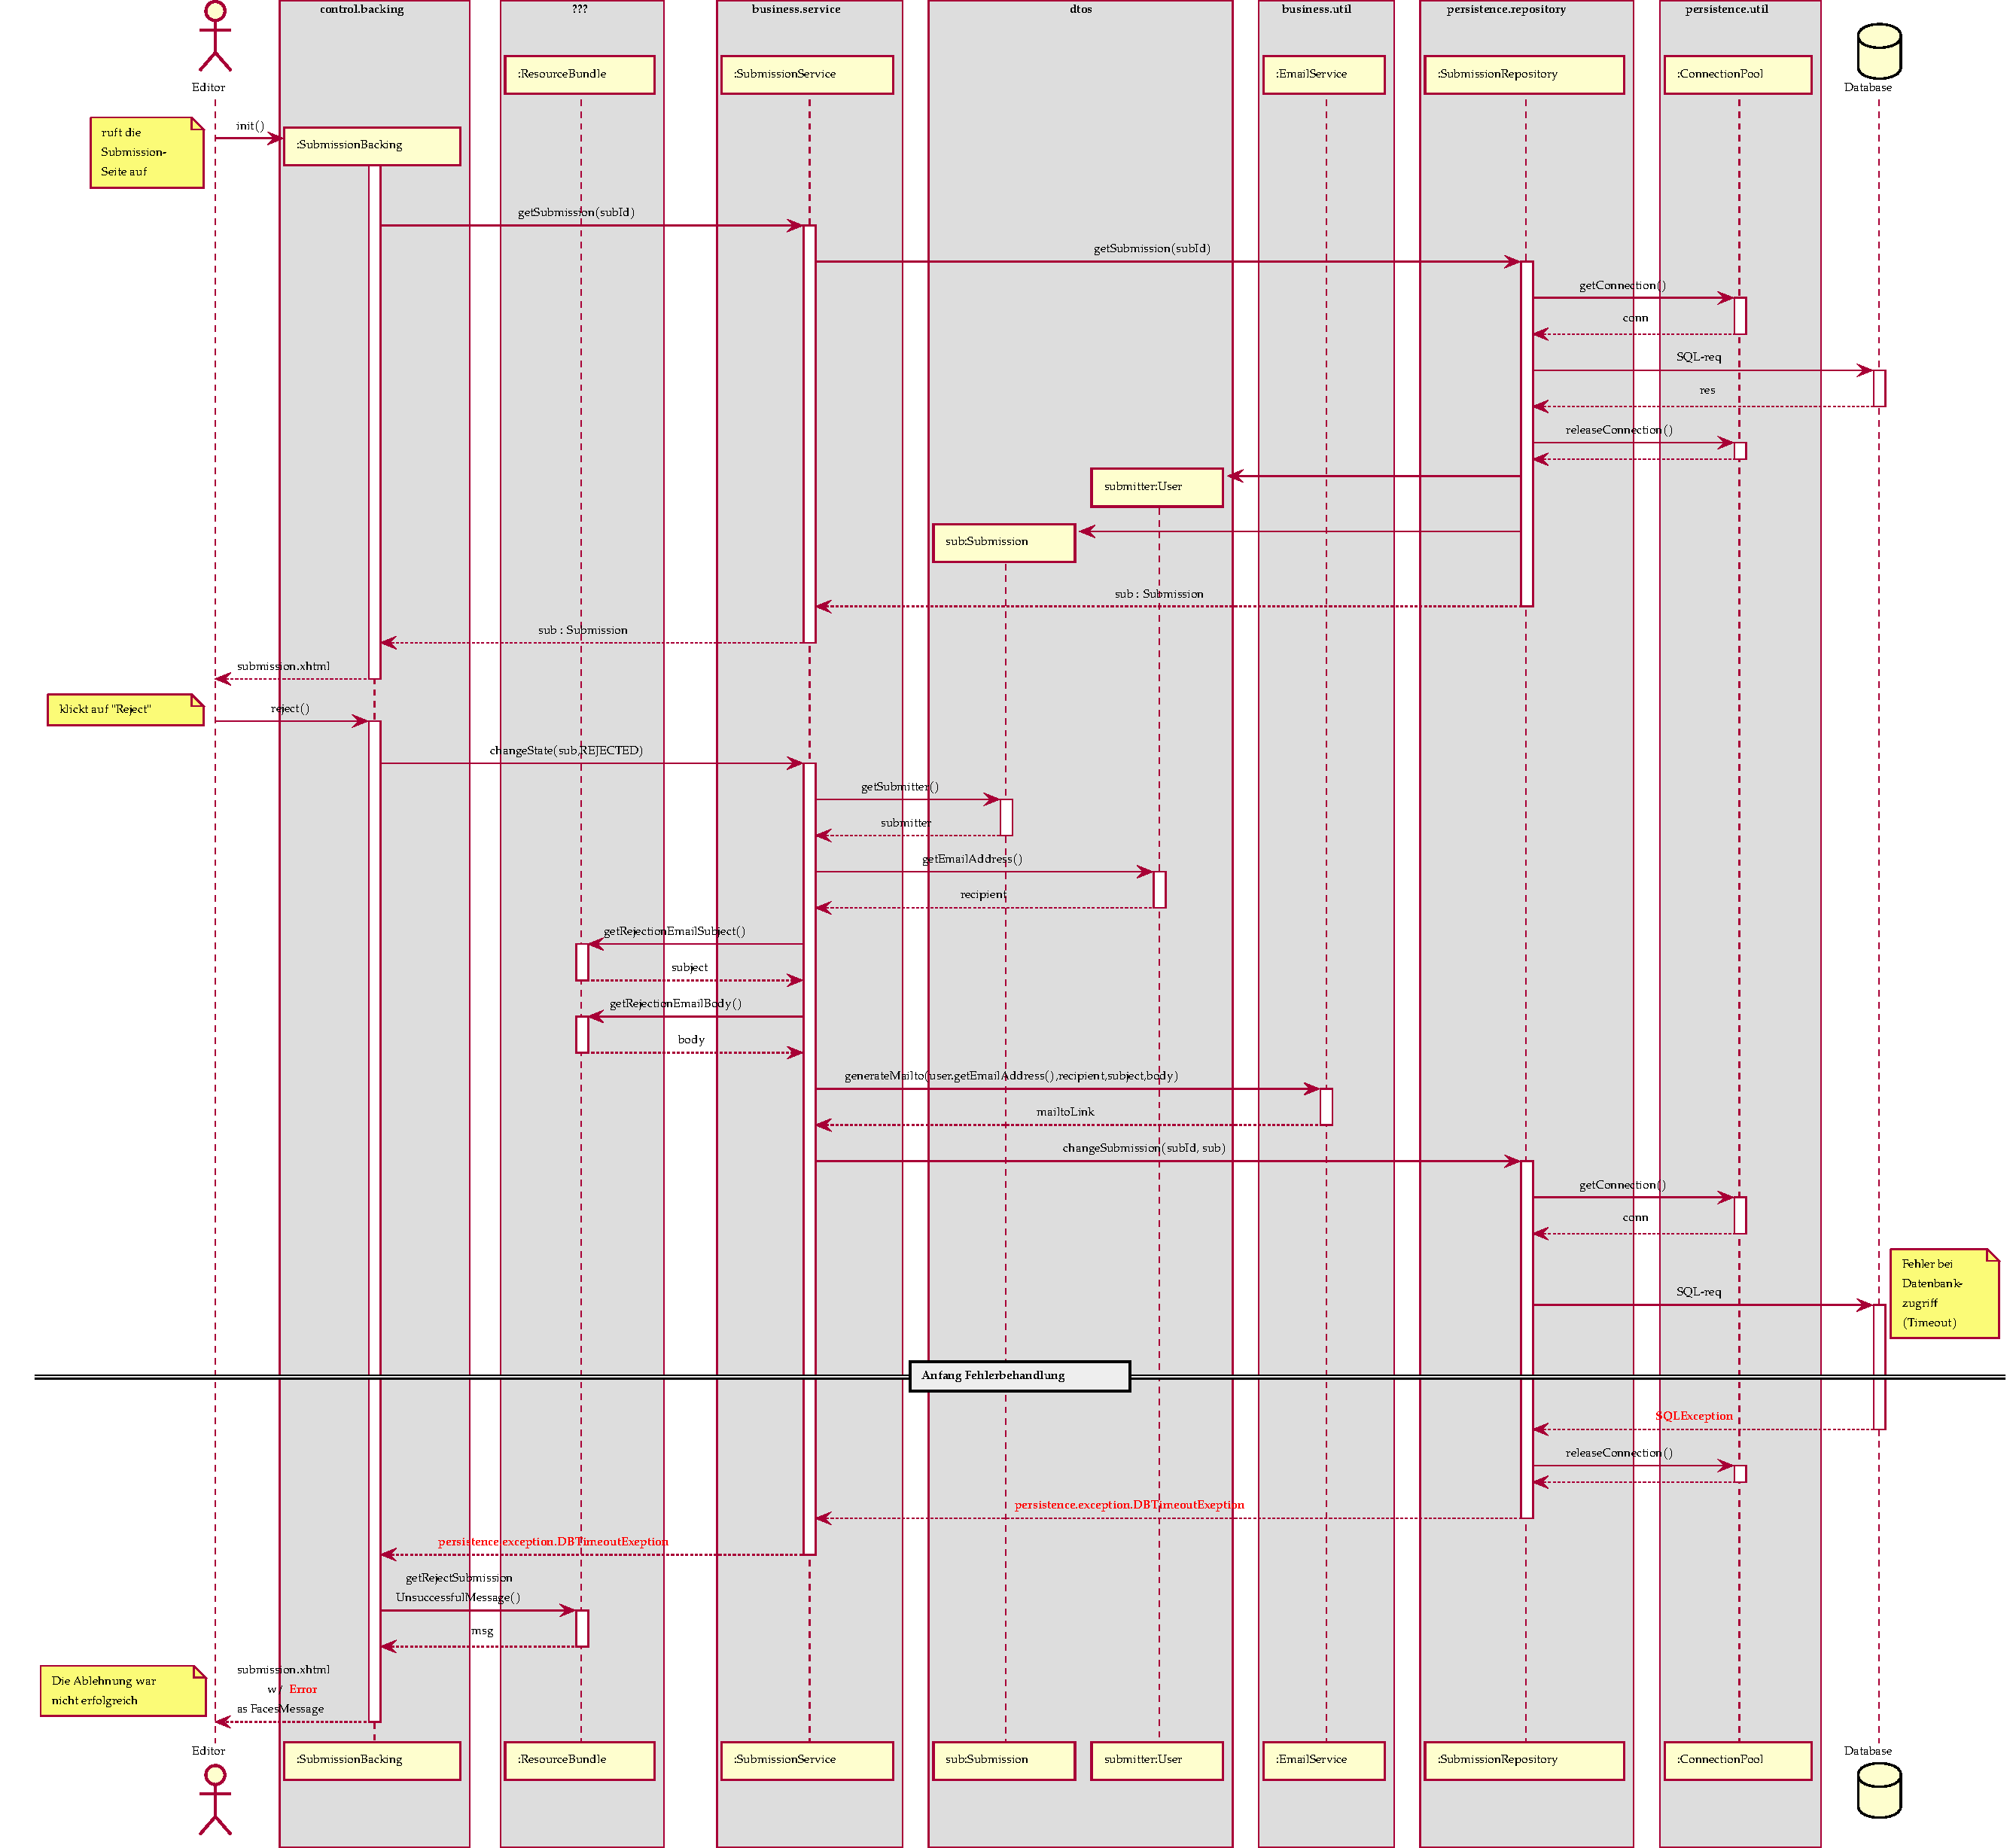
\includegraphics[width=\textwidth]{graphics/reject_submission}
    \caption{Sequenzdiagramm zur Ablehnung einer Einreichung}
    \label{fig:rejection-sequence}
\end{figure}
